\section{Use Case}
\label{sec:casestudy}
% \label{sec:usecase}
% The use case evaluates a batteryless plant sensor such as that of~\cite{cappelle2025} in a simulated cultivation room. The sensor harvests energy at \SI{915}{MHz} and reports over \gls{ble} at \SI{2.4}{GHz}, so the same scenes are traced at both frequencies, and at \SI{5.18}{GHz} for comparison. The metrics follow \cref{sec:metrics}.

% \emph{Crop and Cultivation Environment. }
% The scene is a \SI{5.8}{m} by \SI{5.8}{m} cultivation room with trays on legs, a structural frame, sprayers, windows, a robot, and people. Three plant generations are evaluated, with canopy heights of \SIlist{0.17;0.37;0.68}{m}. The plant materials use the provisional vegetation model of \cref{sec:materials}. \gilles{add picture of a snapshot of the scenario, can be removed later if needed. or reused in previous sections.}

% \emph{Sensor Node and Gateway Locations. }
% Each plant generation is a bed of plants, with nine sensor nodes placed on the plants at positions generated with the scene, between \SI{5}{cm} and \SI{29}{cm} above the growing tray. A single gateway, \SI{2}{m} above the trays near the centre of the room, powers the sensor nodes and collects their reports. Every sensor node was checked for a surface within \SI{1}{cm} in the direction of the gateway, where Sionna RT discards the path segments (\cref{sec:raytracing}); this applies to two of the 27 sensor nodes, both of generation 1, whose gain dropped by up to \SI{40}{dB}, so they are excluded.

% \emph{Simulation and Device Settings. }
% Each scene is traced at \SI{915}{MHz}, \SI{2.437}{GHz}, and \SI{5.18}{GHz} with isotropic, vertically polarised antennas, line of sight, specular reflection, and refraction, up to five interactions per path, and $10^6$ samples per gateway. The gateway provides \SI{30}{dBm} at \SI{915}{MHz}. The \gls{ble} uplink uses \SI{0}{dBm} at the sensor node, a sensitivity of \SI{-95}{dBm} at the gateway, and a \SI{10}{dB} reserve. Two commercial harvesters are compared at the same RF powers (\cref{fig:harvester_efficiency}): the e-peas AEM40940 at \SI{921}{MHz}, designed for low input powers, and the Powercast P1110B at \SI{915}{MHz}, designed for higher ones. Their DC output is modelled by quadratic fits to the datasheet curves from~\cite{ambient6g}. No power is harvested below the lowest datasheet point, at \SI{-20}{dBm} for the AEM40940 and \SI{-5}{dBm} for the P1110B, or where a fit is negative. As the datasheet curves are given at a single output voltage, the time to charge a \SI{346}{\micro\farad} buffer from \SI{0.05}{V} to \SI{4.5}{V} is approximated at constant power as $t=C\,(V_1^2-V_0^2)/(2P_{\mathrm{DC}})$, neglecting leakage.

\label{sec:usecase}
The use case evaluates a batteryless plant sensor such as that of~\cite{cappelle2025} in a simulated cultivation room. The sensor harvests energy at \SI{915}{MHz} and reports over \gls{ble} at \SI{2.437}{GHz}. Four sweeps are run over growth stages 0--4: the carrier frequency (\SI{868}{MHz}, \SI{915}{MHz}, \SI{2.437}{GHz}, and \SI{5.18}{GHz}), the plant species, the gateway density, and the leaf water content.

\emph{Crop and Cultivation Environment. }
The scene is a \SI{4.8}{m} by \SI{4.8}{m} cultivation room with trays on legs, a structural frame, sprayers, and windows (\cref{fig:usecase-paths}). Unless swept, the crop is cherry tomato, whose canopy reaches \SIlist{0.14;0.33;0.56;0.91;1.17}{m} above the tray base in stages 0 to 4. Leaves use the provisional vegetation model of \cref{sec:materials} with \SI{80}{\percent} water content and a slab thickness of \SI{0.3}{mm}; stems are omitted. The concrete floor uses the ITU-R P.2040 model~\cite{itu2040}, extrapolated below \SI{1}{GHz}.

\begin{figure}[hbtp]
    \centering
    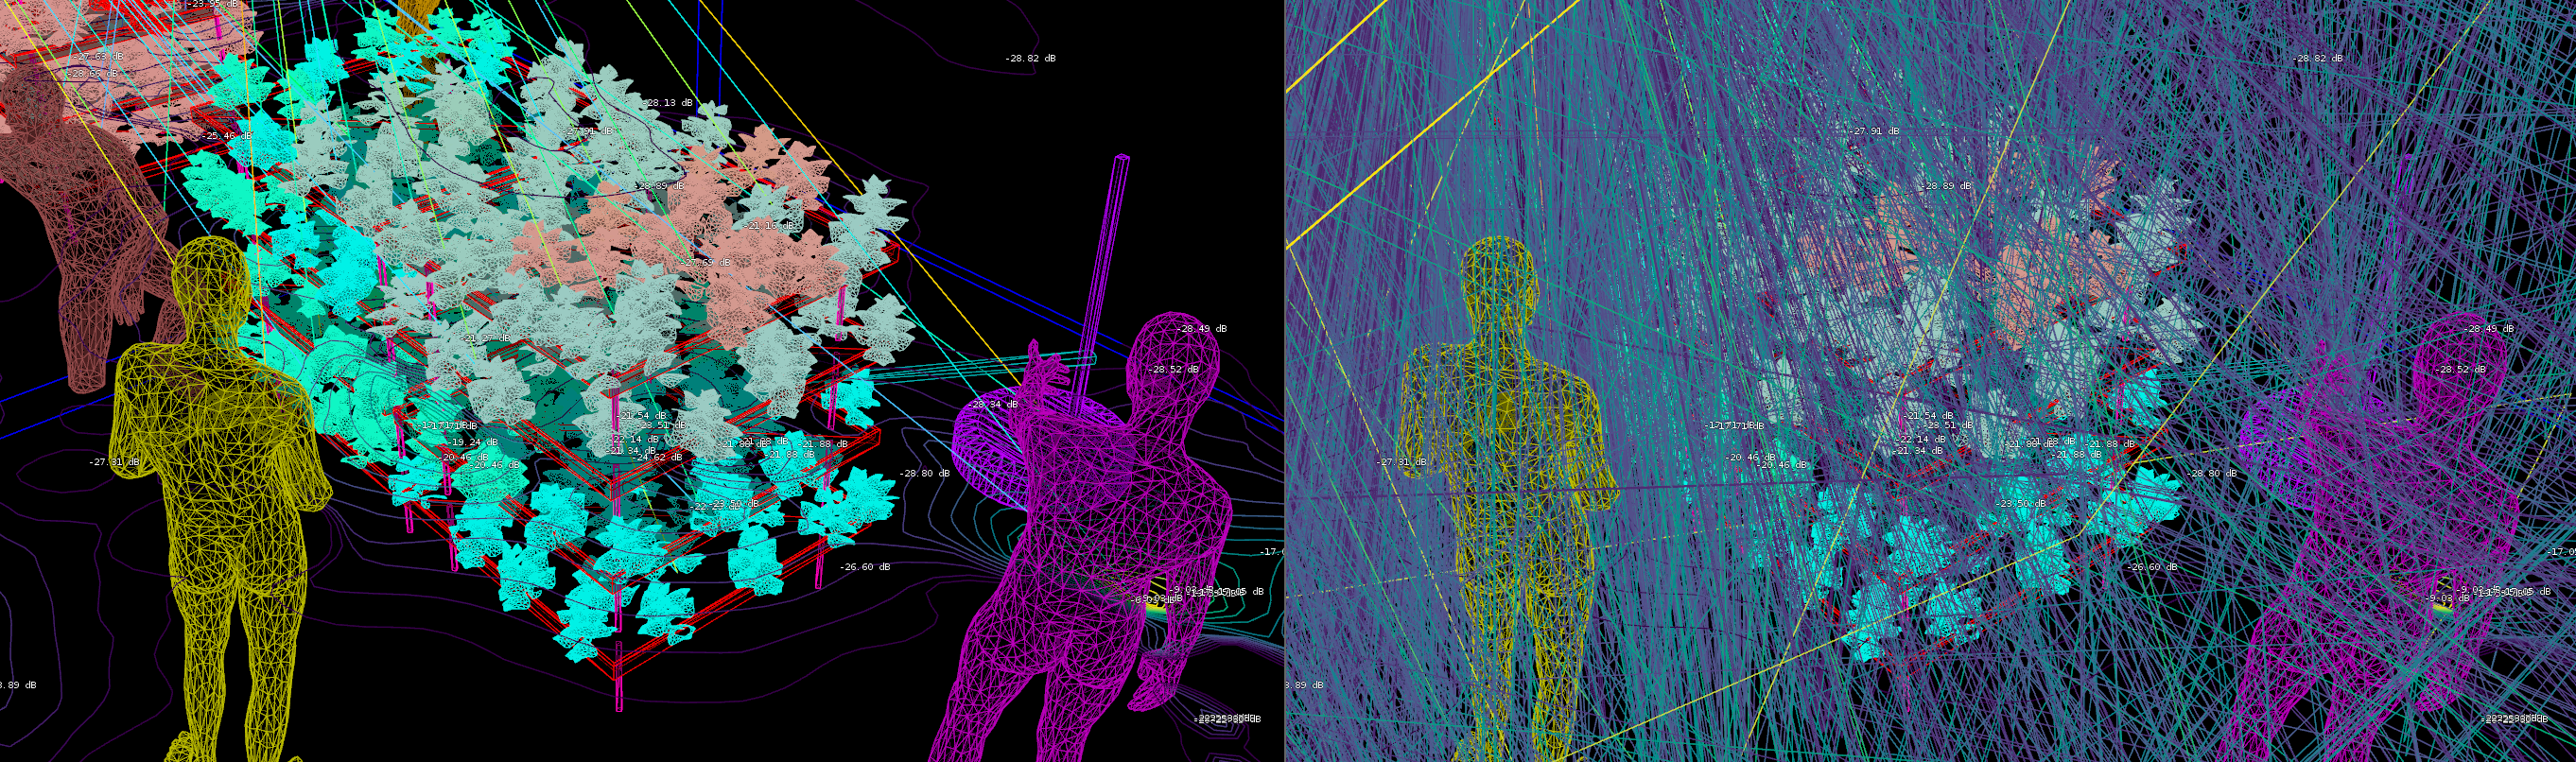
\includegraphics[width=0.98\linewidth]{figures/screenshots/snapshot combined.png}%
    % 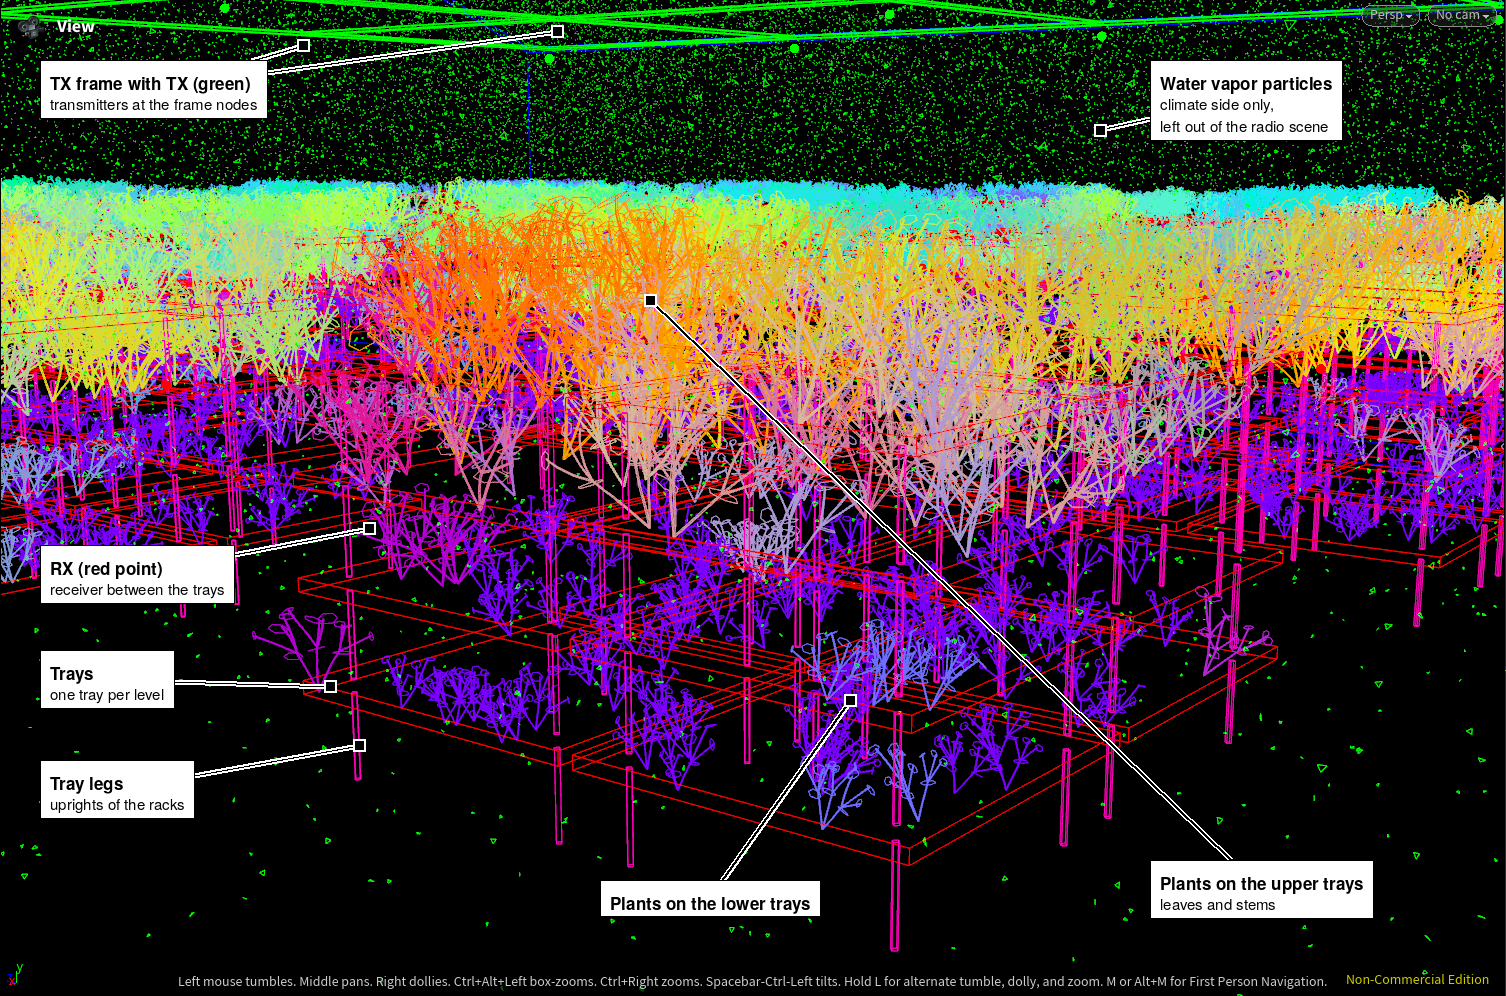
\includegraphics[width=0.5\linewidth]{figures/procedural/annotated_00bbc1c9.png}
\caption{An example cultivation scene, here with people, without and with the traced propagation paths, coloured by path delay $\tau$.}
\label{fig:usecase-paths}
\end{figure}

\emph{Sensor Node and Gateway Locations. }
Each stage is a bed of 18 plants with one sensor node per plant, attached \SI{2}{cm} from leaves, stems, and trays, so its own plant does not trigger the \SI{1}{cm} segment limit (\cref{sec:solver}). Sensor nodes with another surface within \SI{1}{cm} towards a gateway are excluded, up to three of the 18 in stage 4. Gateways \SI{2}{m} above the trays, facing down, power the sensor nodes and collect their reports: one by default, and 1 to 23 when the density is swept from one per \SI{30}{m^2} to one per \SI{1}{m^2}.

\emph{Simulation and Device Settings. }
Each scene is traced with line of sight, specular reflection, refraction, and diffraction, up to eight interactions per path, $3\times10^{6}$ samples and at most $10^{5}$ paths per transmitter, and seed 42. The sensor nodes use half-wave dipoles aligned with the main stem; the gateway uses a vertically polarised TR 38.901 element pattern. Sensor nodes are traced as transmitters; with fixed antennas, reciprocity lets the same gains serve the power transfer and the uplink. The gateways provide \SI{30}{dBm} in total at \SI{915}{MHz}; several gateways transmit coherently with maximum-ratio transmission (\cref{sec:returned}). The \gls{ble} uplink uses \SI{0}{dBm} at the sensor node, a sensitivity of \SI{-95}{dBm} at the gateway, and a \SI{10}{dB} reserve. Two commercial harvesters are compared at the same RF powers (\cref{fig:harvester_efficiency}): the e-peas AEM40940, designed for low input powers, and the Powercast P1110B, designed for higher ones. Their DC output is modelled by quadratic fits to the curves of~\cite{ambient6g}. No power is harvested below the lowest data point, at \SI{-20}{dBm} for the AEM40940 and \SI{-5}{dBm} for the P1110B, or where a fit is negative. As the curves are given at a single output voltage, the time to charge a \SI{346}{\micro\farad} buffer from \SI{0.05}{V} to the maximum storage voltage of \SI{4.5}{V} for the AEM40940, and to the maximum output voltage of \SI{4.2}{V} for the P1110B, is approximated at constant power as $t=C\,(V_1^2-V_0^2)/(2P_{\mathrm{DC}})$, neglecting leakage and cold start.

% , $P_{\mathrm{DC}}=aP_{\mathrm{RF}}^2+bP_{\mathrm{RF}}+c$ with both powers in microwatts, obtained by minimising the squared relative error: $(a,b,c)=(-2.04\cdot10^{-5},\,0.268,\,-2.19)$ for the AEM40940 and $(-1.81\cdot10^{-6},\,0.701,\,-189)$ for the P1110B. The fits are used within the datasheet range, which starts at \SI{-20}{dBm} for the AEM40940 and at \SI{-5}{dBm} for the P1110B; below it, and where a fit is negative, no power is harvested. Leakage and storage losses are not included.

% Read the original CSV directly; select each curve by its harvester column.
% text indicator handles commas inside the quoted series descriptions.
% RF input power is read directly from the level_dbm column.
\begin{figure}[t]
\centering
\pgfplotstableread[col sep=comma,text indicator="]
  {figures/harvester-chart-data.csv}\harvesterchartdata
\begin{tikzpicture}
\pgfplotsset{
  harvester series/.style={
    x filter/.code={
      \pgfplotstablegetelem{\coordindex}{harvester}\of\harvesterchartdata
      \edef\currentharvester{\pgfplotsretval}%
      \edef\selectedharvester{#1}%
      \ifnum\pdfstrcmp{\currentharvester}{\selectedharvester}=0
      \else
        \def\pgfmathresult{nan}%
      \fi
    },
    unbounded coords=discard,
    filter discard warning=false,
  },
}
\begin{axis}[
  width=\columnwidth,
  height=3.5cm,
  font=\footnotesize,
  xlabel={RF input power (dBm)},
  ylabel={Efficiency (\%)},
  label style={font=\footnotesize},
  tick label style={font=\scriptsize},
  xmin=-22, xmax=10,
  ymin=0, ymax=70,
  xtick={-25,-20,-15,-10,-5,0,5,10},
  ytick={0,20,...,60},
  grid=major,
  major grid style={draw=black!12},
  axis line style={draw=black!70},
  tick align=outside,
  tick pos=left,
  legend cell align=left,
  legend style={
    at={(0.03,0.97)}, anchor=north west,
    font=\scriptsize,
    draw=none, fill=white, fill opacity=0.9, text opacity=1,
    nodes={scale=1,transform shape},
    row sep=1pt,
  },
]
\addplot+[line width=0.9pt,draw={rgb,255:red,117;green,112;blue,179},solid,mark=*,mark size=1.3pt,harvester series=AEM40940]
table[x=level_dbm,y=efficiency] {\harvesterchartdata};
\addlegendentry{AEM40940}

\addplot+[line width=0.9pt,draw={rgb,255:red,217;green,95;blue,2},dashed,mark=square*,mark repeat=7,mark size=1.4pt,harvester series=P1110B]
table[x=level_dbm,y=efficiency] {\harvesterchartdata};
\addlegendentry{P1110B}

% \addplot+[line width=0.9pt,draw={rgb,255:red,27;green,158;blue,119},densely dotted,mark=triangle*,mark repeat=7,mark size=1.6pt,harvester series=SMS7630005LF]
% table[x=level_dbm,y=efficiency] {\harvesterchartdata};
% \addlegendentry{Low-power rectifier}

\end{axis}
\end{tikzpicture}
\caption{RF-to-DC efficiencies from the AMBIENT-6G harvester dataset~\cite{ambient6g}, at \SI{921}{MHz} for the AEM40940 and \SI{915}{MHz} for the P1110B.}
\label{fig:harvester_efficiency}
\end{figure}


\subsection{Deployment Results}

\begin{table}[t]
\caption{Results per growth stage for cherry tomato with one gateway, for the same 18 sensor nodes in every stage: median and worst path gain and median RF power at \SI{915}{MHz} (which, unlike the gain, includes fast fading), worst \gls{ble} margin at \SI{2.437}{GHz} beyond the \SI{10}{dB} reserve, and the number of sensor nodes whose harvester charges the buffer within one hour. One sensor node of stage 4 has no path to the gateway; it counts as not charged and is left out of the worst gain and margin.}
\label{tab:usecase}
\centering\footnotesize
\setlength{\tabcolsep}{3.5pt}
\begin{tabular}{@{}rrrrrrr@{}}
\toprule
 & \multicolumn{2}{c}{Gain (dB)} & \gls{ble} & $P_{\mathrm{RF}}$ & \multicolumn{2}{c}{Within \SI{1}{h} (of 18)} \\
\cmidrule(lr){2-3}\cmidrule(l){6-7}
Stage & Median & Worst & (dB) & (dBm) & AEM40940 & P1110B \\
\midrule
0 & $-36.1$ & $-48.7$  & $24.3$  & $-6.1$  & 17 & 9 \\
1 & $-47.9$ & $-57.8$  & $14.4$  & $-19.9$ & 8  & 1 \\
2 & $-51.4$ & $-59.2$  & $8.7$   & $-21.6$ & 7  & 1 \\
3 & $-52.5$ & $-66.9$  & $7.6$   & $-24.2$ & 5  & 1 \\
4 & $-64.3$ & $-102.0$ & $-20.4$ & $-36.9$ & 1  & 0 \\
\bottomrule
\end{tabular}
\end{table}

\Cref{tab:usecase} summarises the growth stages of the frequency sweep at \SI{915}{MHz}. Growth dominates: from stage 0 to stage 4, the median gain drops by \SI{28}{dB} and the median RF power from \SI{-6.1}{dBm} to \SI{-36.9}{dBm}. Over all stages, the median gain is \SI{-52.0}{dB} at \SI{915}{MHz} (\SI{-51.4}{dB} at \SI{868}{MHz}) and drops by \SI{10.1}{dB} at \SI{2.437}{GHz} and by \SI{18.3}{dB} at \SI{5.18}{GHz}, which is \SIlist{1.6;3.3}{dB} more than free-space scaling: the canopy attenuates more at higher frequencies.

Energy limits the sensor nodes first, and it depends on the harvester. With the AEM40940, whose data start at \SI{-20}{dBm}, 17 of the 18 sensor nodes charge the buffer within one hour in stage 0, but only 8 in stage 1 and a single one in stage 4. The P1110B needs \SI{-5}{dBm} and charges 9 sensor nodes in stage 0 and at most one in the later stages; above this threshold it charges the buffer within minutes, so its counts are set by the input threshold, not by the target voltage. The \gls{ble} uplink keeps at least \SI{7.6}{dB} beyond the reserve up to stage 3, but in stage 4 the worst sensor node falls \SI{20.4}{dB} short and one has no path at all.

More gateways help while the canopy is open. With 23 coherently combined gateways, all 18 sensor nodes charge within one hour with the AEM40940 in stages 0 to 2, against 17, 9, and 7 with one gateway in the same sweep, but in stage 4 only 2 of the 16 sensor nodes that are not excluded do: the dense canopy, not the number of gateways, then limits power delivery. The species matters as much as the stage: the median RF power under butterhead lettuce stays near \SI{-17}{dBm} in every stage, whereas it falls by \SI{11}{dB} for sweet basil, \SI{18}{dB} for strawberry, and \SI{29}{dB} for cherry tomato. Leaf water content between \SIlist{20;90}{\percent} changes the median gain by at most \SI{2}{dB}, as \SI{0.3}{mm} leaves are electrically thin, and the number of charged sensor nodes by at most two. Runs with identical inputs and seed are not bit-identical on the GPU; between such runs, the count differs by at most one sensor node.

